\chapter{DESCRIÇÃO DA TÉCNICA} \label{cap:tecnica}

Neste capítulo objetiva-se a descrição da técnica desenvolvida neste trabalho.

Inicialmente é apresentado o funcionamento da técnica quanto a forma como o mapeamento dinâmico é realizado e, posteriormente, como o intervalo de busca é calculado a partir do mapeamento. Em seguida a implementação da técnica é descrita juntamente com o diagrama de módulos atualizado do simulador e os parâmetros que podem ser ajustados dentro do ambiente simulado. Por fim, o capítulo é finalizado com uma conclusão a cerca dos assuntos debatidos.

\section{Funcionamento}

Como apresentado na subseção \ref{sec:definicoes}, as DTNs dependem das oportunidades de contato para a retransmissão de mensagens. Por sua vez, os contatos são influenciados diretamente pelo intervalo de busca por dispositivos próximos, visto que durante um período de espera um nó pode acabar não contatando outros que estava próximos. A partir daí, o gerenciamento do intervalo de busca de acordo com a probabilidade de contato numa determinada localização permite o ajusto dinâmico do intervalo fixo de espera de 32 segundos proposto por \cite{denis_artigo}.

O comportamento praticamente estocástico dos dispositivos, como os das moléculas de sacarose dissolvendo-se em água, torna a previsibilidade da localização dos contatos dificultosa em diversos cenários, como o das Redes Móveis Ad Hoc e o ZebraNet. Todavia, a concentração pode ser calculada por meio de um mapeamento dinâmico utilizando módulos de GPS dos dispositivos.

\subsection{O Mapeamento Dinâmico}

Inicialmente, uma divisão do mapa em regiões de igual tamanho é realizada. A partir daí, ao estabelecerem contato, os dispositivos envolvidos registram este em uma \emph{Tabela de Mapeamento de Regiões} (TMR). É por meio dessa tabela que cada nó tem uma visão global do mapa, pois sempre armazenam as quantidades de contatos registrados em cada uma das regiões pelas quais cada nó passou. Ao registrar um contato, é feita uma consulta GPS para determinar com precisão em que região o nó se encontra e contabilizar esse evento.

Após o registro do contato na tabela, os nós trocam suas TMRs para dinamizar o mapeamento e permitir que tenham acesso a dados de regiões pelas quais eles ainda não passaram. É passível de afirmação que o compartilhamento das TMRs implementa a prosa descrita na subseção \ref{subsec:gradientes_desafios}, onde dois nós, educadamente, compartilham um com o outro as informações que possuem acerca das regiões por onde passaram.

É de grande importância o estudo quanto a forma de mesclagem das tabelas de mapeamento. Durante o desenvolvimento deste trabalho foram consideradas três formas para tal, sendo elas:

\begin{itemize}
    \item \textbf{Mesclagem por Soma:} Nesta modalidade de mesclagem, para cada registro do nó contatado, se o dispositivo que recebeu a tabela, já possui alguma informação do registro é realizada uma soma dos valores. Caso contrário, o valor é adicionado a um novo registro na tabela. Em suma esta estratégia parece interessante, mas, durante as simulações, foi percebido que o comportamento cíclico de alguns nós causa a geração de registros extremamente discrepantes com relação ao comportamento real da rede, além de, após longos períodos de simulação, ocorrerem problemas com \emph{overflow} de variáveis mesmo quando utilizando \emph{64bits} de tamanho;
    \item \textbf{Mesclagem Incremental:} Ao realizar a mesclagem das tabelas, para cada registro do nó contatado, se o dispositivo já possui algum registro daquela região, é feito um incremento de um no registro local. Caso contrário, o valor é copiado para um novo registro na tabela. Esta abordagem não se mostrou satisfatória durante as simulações pois não conseguiu representar de forma satisfatória o comportamento real do mapa de regiões, ocorrendo momentos em que os valores ficaram totalmente incoerentes com a realidade;
    \item \textbf{Mesclagem por Substituição do Maior:} Nesta forma de mesclagem, para cada registro do outro nó, caso já exista um registro na tabela local e este seja menor que o do outro nó, é realizada a substituição. Caso não exista registro local, o valor é copiado. Caso contrário, ou seja, o valor local é maior que o do outro dispositivo, nada é feito. Esta forma de mesclagem foi a que melhor conseguiu representar o mapa regiões real, apresentando proporções coerentes com o comportamento real da rede.
\end{itemize}

Neste trabalho é considerada a mesclagem por meio da substituição do maior elemento devido ao fato de ter apresentado, durante as simulações, melhor representação do comportamento real da rede num ambiente onde o mapa é construído de forma independente e dinâmica.

Dados dois nós \emph{A} e \emph{B} localizados próximos e com o nó \emph{A} realizando buscas, o comportamento do mapeamento dinâmico é descrito pela Figura \ref{mapeamento}. É importante ressaltar que, neste trabalho, não foi considerada a sobrecarga gerada pela troca das TMRs.

\begin{figure}[htp!]
\centering
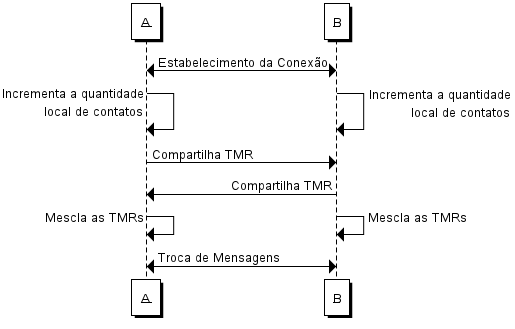
\includegraphics[width=0.75\textwidth]{figuras/cap_4/mapeamento.png}
\caption{Diagrama de Sequência do Mapeamento Dinâmico utilizando as TMRs}
\label{mapeamento}
\end{figure}

\subsection{Dinamização do Intervalo de Busca}
\label{sec:dinamizacao_intervalo_busca}
Tendo as Tabelas de Mapeamento de Regiões construídas dinamicamente, os dispositivos podem calcular livremente a probabilidade de contato em cada uma das regiões definidas previamente. Como pode ser visto em \cite{hazzan2013fundamentos}, a probabilidade de um evento $A$ ocorrer ($P(A)$), pode ser descrita por:

\begin{equation}
P(A)=\frac{n(A)}{n(\Omega)}
\end{equation}

Onde $n(A)$ é a quantidade de casos favoráveis a $A$ e $n(\Omega)$ é o número de resultados do experimento.

Tendo noção da probabilidade de contato $P(r)$ de um nó encontrar outro na região $r$, há duas decisões que um nó pode tomar: Aumentar ou diminuir o intervalo de buscas. Se um nó está em uma região com alta probabilidade de contato, este pode gastar mais a sua bateria visando aproveitar melhor as oportunidades daquela região. Caso a probabilidade seja muito pequena, o nó possui menor chance de tirar proveito de sua bateria, fazendo mais sentido economizá-la para um momento mais oportuno.

Observa-se então que, a concentração estimada em uma determinada região é, na verdade, a probabilidade de contato nessa localidade. A justificativa para isto baseia-se na grande importância dos contatos para as DTNs e na limitada visão que os dispositivos possuem quanto a quantidade de dispositivos próximos, visto hardware limitado que geralmente possuem. Além disso, regiões com altas taxas de contatos tendem a ser mais frequentadas por muitos dispositivos, influenciando diretamente na concentração efetiva da localidade.

Existe, entre a concentração, ou probabilidade de contado, e o intervalo de busca, um relacionamento de proporcionalidade inversa, ou seja, quanto maior a probabilidade, menor o intervalo de busca, e, quanto menor a probabilidade, maior o intervalo de busca. Sendo assim, é preciso descrever este relacionamento por meio de uma equação que o representa corretamente.

A proposta deste trabalho é que, dado um intervalo mínimo de busca $Im$, um intervalo máximo $IM$ pré-definidos e a probabilidade de contato na região em que o nó se encontra $P(r)$, pode-se descrever o intervalo de busca dito ideal $Ir$ como:

\begin{equation}
Ir=Im + (1-P(r))(IM-Im)
\label{eq_intervalo_ideal}
\end{equation}

O relacionamento de proporcionalidade inversa é descrito pelo termo $1-P(r)$, este pode ainda ser entendido como a probabilidade do contato não ocorrer \cite{hazzan2013fundamentos}. O termo $IM-Im$, quando multiplicado por $1-P(r)$ e posteriormente somado a $Im$, garante queo intervalo $Ir$ seja no máximo igual a $IM$  e no mínimo igual a $Im$.

O intervalo de busca ideal da região atual de um determinado nó da rede é calculado sempre quando este inicia um novo ciclo de busca que, por sua vez, nada mais é do que um período de procura por nós seguido de um intervalo de espera $Ir$ da região $r$ onde ele se encontra.

Quando a rede inicia sua operação, é notável que, durante certo período de tempo, os nós não possuem dados em suas TMRs ou estes ainda não são fieis ao comportamento estimado da rede. Para contornar este problema, foi proposto que a técnica passasse por um período de aquecimento, ou \emph{warmup time}, que é um período pré-definido onde os nós não fazem uso de suas TMRs e definem seus intervalos de busca como sendo o intervalo ideal de 32 segundos proposto por \cite{denis_artigo}.

Ainda existe o caso onde um determinado nó pode não ter dados sobre os contatos registrados na região onde ele se encontra. Para este caso, foi considerado o intervalo de busca de 32 segundos.

O diagrama da Figura \ref{diagrama} descreve de forma sucinta o funcionamento da técnica quanto a dinamização do intervalo entre as buscas por dispositivos.

\begin{figure}[htp!]
\centering
\includegraphics[width=0.75\textwidth]{figuras/cap_4/diagrama.png}
\caption{Diagrama de fluxo da dinamização do intervalo de busca}
\label{diagrama}
\end{figure}

\section{Descrição da Implementação}

A implementação da técnica dentro do simulador The ONE passou por duas etapas principais e importantes de serem descritas neste trabalho: a preparação do simulador e o desenvolvimento efetivo da técnica.

\subsection{Preparação do Simulador The ONE}

Antes do desenvolvimento efetivo da técnica, foi preciso preparar o simulador. É nesta etapa que o módulo de GPS foi implementado e sua respectiva incorporação com o módulo de energia foi feita.

O módulo de GPS nada mais é que uma classe \emph{GPSModule} integrada à classe \emph{DTNHost} que, por sua vez, é responsável por representar cada nó da rede simulada. 

O \emph{GPSModule} possui dois modos de operação. São eles:

\begin{itemize}
    \item \textbf{Com consumo:} É modo utilizado para contabilização de energia consumida pelo dispositivo de GPS integrado aos hosts. A cada consulta GPS o \emph{GPSModule} se encarrega de notificar ao módulo de energia \emph{EnergyModel} que este foi utilizado e consumiu a bateria.
    \item \textbf{Sem consumo:} É o modo utilizado para simulações quando não se deseja contabilizar o consumo do dispositivo de GPS.
\end{itemize}

Devido ao fato dos dispositivos GPS também serem responsáveis pelo consumo das baterias, o módulo desenvolvido também é integrado ao módulo de energia do simulador. A contabilização do consumo é feita a cada consulta GPS realizada pelo dispositivo a partir da chamada ao método \emph{reduceEnergy} explanado na subseção \ref{modulo_energia}.

A forma como o módulo foi implementado permite que o usuário defina padrões de consumo para cada um grupo de nós. Como exemplo, é possível criar dois grupos um para \emph{smartphones} e outro para carros e definir um consumo diferente de energia para cada um deles. Caso seja desejado, é possível ainda definir um consumo global, onde todos os nós respeitam um único padrão de consumo.

A utilização do módulo necessita da definição da quantidade de energia que é consumida pelo dispositivo GPS em cada consulta. Essa configuração se dá por meio da propriedade \emph{gpsScanEnergy} dentro do arquivo de configurações do simulador apresentado na subseção \ref{subsec:arquivo_configuracao}. Em caso da omissão dessa linha de configuração, o simulador entenderá que modo de operação é o \emph{sem consumo} e, consequentemente, não contabilizará o consumo de energia por parte dos dispositivos GPS.

A Figura \ref{gps_config} apresenta um exemplo de configuração onde todos os dispositivos são configurados para consumirem 154,6mW em cada consulta GPS.

\begin{figure}[htp!]
\centering
\lstinputlisting[language=Java]{codigos/gps_config.txt}
\caption{Exemplo de configuração do consumo do módulo de GPS.}
\label{gps_config}
\end{figure}

\subsection{Desenvolvimento da Técnica}

A técnica desenvolvida teve seu foco principal na modelagem da \emph{Tabela de Mapeamento de Regiões}, no modelo de ajuste de busca e na integração deles com o simulador.

A TMR foi implementada pela classe \emph{ConcentrationMap}, que, por sua vez, utiliza uma tabela de dispersão para armazenar as informações das regiões definidas por meio do tamanho base \emph{RegionLength}. Esta estratégia de armazenamento permite economia de memória, visto que apenas as regiões com dados conhecidos são armazenadas pelo dispositivo.

O modelo de ajuste de busca, definido pelo \emph{ScanAdjustmentModel}, é responsável pela dinamização do intervalo de busca por dispositivos. É nele que se encontra o método \emph{getBestScanTime}, responsável por realizar o cálculo da equação \ref{eq_intervalo_ideal}, apresentada na subseção \ref{sec:dinamizacao_intervalo_busca}, e retornar o intervalo apropriado para a região em que o nó se encontra. Além dos intervalos mínimos e máximos de busca, representados pelos parâmetros \emph{MinScanInterval} e \emph{MaxScanInterval}, respectivamente, o método também recebe o parâmetro \emph{DefaultScanInterval}, que, por sua vez, representa o intervalo de busca padrão a ser utilizado quando em \emph{warmup time} ou quando o dispositivo não possui dados sobre a região onde se encontra.

É importante ressaltar que, o intervalo padrão pode ser ajustado livremente pelo usuário, mas, neste trabalho, considerou-se apenas o intervalo ideal proposto por \cite{denis_artigo}, ou seja, 32 segundos, como visto na Figura \ref{diagrama}.

Tendo a TMR e o modelo de ajuste de busca implementados, foi necessário integrá-los ao simulador. Para isso a interface de rede dos nós, representada pela classe \emph{NetworkInterface}, precisou ser alterada. Em suma, apenas o método \emph{isScanning} foi modificado para utilizar o intervalo de busca apropriado (retornado pelo método \emph{getBestScanTime}) quando detecta que um novo ciclo de busca foi iniciado.

Dentro da arquitetura do simulador, o resultado das alterações feitas é apresentado no diagrama da Figura \ref{theOne_modificado}. A técnica em si, foi implementada dentro do módulo \emph{Conectivity and Data} e é representada em laranja como \emph{TMR and GPS module}.

A Figura \ref{tecnica_config} exibe um exemplo de configuração para todos os dispositivos dos parâmetros \emph{DefaultScanInterval}, \emph{MinScanInterval}, \emph{MaxScanInterval}, \emph{RegionLength} e \emph{AdjustmentWarmup}.

A Tabela \ref{parametros_ajustaveis} apresenta individualmente os parâmetros da técnica que podem ser ajustados para a descrição do cenário de simulação dentro do arquivo de configurações do simulador apresentado na Subseção \ref{subsec:arquivo_configuracao}.
\begin{figure}[htp!]
\centering
\includegraphics[width=1\textwidth]{figuras/cap_4/TheONEArchtecture_modificada.png}
\caption{Diagrama de fluxo da dinamização do intervalo de busca}
\label{theOne_modificado}
\end{figure}

\begin{figure}[htp!]
\centering
\lstinputlisting[language=Java]{codigos/tecnica_config.txt}
\caption{Configuração dos parâmetros de funcionamento da técnica.}
\label{tecnica_config}
\end{figure}


\begin{table}[H]
\centering
\caption{Parâmetros ajustáveis da técnica.}
\begin{tabular}{|l|l|l|}
\hline
\textbf{Parâmetro}        & \textbf{Tipo}   & \textbf{Ação}                                                      \\ \hline
GpsScanEnergy    & double & \begin{tabular}[x]{@{}l@{}}Define a quantidade de energia gasta a cada busca\\de GPS.\end{tabular} \\ \hline
MinScanInterval  & double & Define o intervalo mínimo de busca.                       \\ \hline
MaxScanInterval  & double & Define o intervalo máximo de busca.                       \\ \hline
DefaultScanInterval  & double & Define o intervalo padrão de busca.                       \\ \hline
AdjustmentWarmup & int    & Define o tempo de aquecimento da técnica.                 \\ \hline
RegionLength     & double & Define o tamanho das regiões.                             \\ \hline
\end{tabular}
\label{parametros_ajustaveis}
\end{table}


\section{Conclusão do Capítulo}

Neste capítulo foi apresentado o funcionamento da técnica desenvolvida e como esta foi implementada dentro do simulador The ONE. Além disso foram apresentados os parâmetros que a técnica permite que sejam alterados.

A partir do momento em que a técnica foi finalizada, o próximo passo é demonstrar seu comportamento nos cenários de teste escolhidos, permitindo avaliar os dados coletados e, finalmente, determinar se a sua aplicabilidade num ambiente real é viável ou não. Tal demonstração e avaliação são apresentadas no capítulo \ref{cap:testes}.